\scanpage{25}
\figure{\handwritten{%
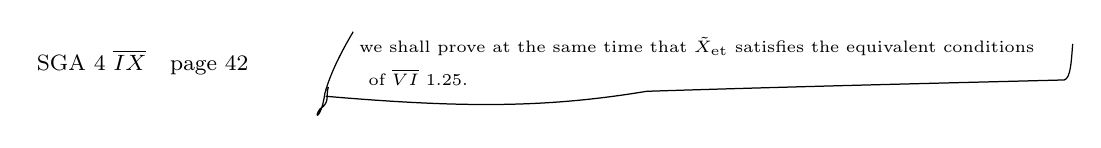
\begin{tikzpicture}[x=.009cm,y=-.009cm,font=\fontsize{8}{9}\selectfont]
\node[anchor=base west] at (160,83) {SGA 4 \(\overline{\text{\uline{IX}}}\)\quad page 42};
\node[anchor=base west,font=\fontsize{6.5}{8}\selectfont] at (615,57) {we shall prove at the same time that $\tilde{X}_{\mathrm{et}}$ satisfies the equivalent conditions};
\node[anchor=base west,font=\fontsize{6.5}{8}\selectfont] at (628,104) {of \(\overline{\text{\uline{VI}}}\) 1.25.};
\draw[line width=.45pt] (620,28) .. controls (601,60) and (587,89) .. (580,115)
 .. controls (575,151) and (563,151) .. (573,137)
 .. controls (588,128) and (581,117) .. (585,106);
\draw[line width=.45pt] (581,119) .. controls (779,136) and (895,135) .. (1034,112)
 .. controls (1254,105) and (1468,100) .. (1623,96)
 .. controls (1632,94) and (1633,70) .. (1635,45);
\end{tikzpicture}}}

\handwritten{(*) (Note for page 8.) Let us prove that the notion of constructibility 2.3 for a sheaf of sets $F$ coincides with that of \(\overline{\text{\uline{VI}}}\) 1.9.3. \deleted{Let} The \deleted{indeed $C$ the \unsure{case}}\inserted{question being} local on $X$, we may assume $X$ affine \inserted{hence ``coherent'', i.e.} quasi-compact and quasi-separated. \deleted{Let $C$ be the category \unsure{Let $C(C')$ be the subcategory|Let $(C')$ be the subcategory}} \deleted{I must then prove that $F$ is constructible} Let $C$ (resp. $C'$) be the \deleted{\unsure{full|quasi}}\inserted{strictly} full subcategory of $\tilde{X}_{\text{ét}}$ consisting of the $F$ constructible in the sense of 2.3, \deleted{\illegible{1}} \inserted{(resp. in the sense of \(\overline{\text{\uline{VI}}}\) 1.9.3), it}}

% The opening conclusion shares the upper-left space of the cancellation graphic.
% The long paths, enclosing edges and nested cross-hatching below are source cancellation marks.

\figure{\handwritten{%
\begin{tikzpicture}[x=.009cm,y=-.009cm,font=\fontsize{6.5}{8}\selectfont]
\node[anchor=base west,rotate=4] at (215,526) {must be proved};
\node[anchor=base west,rotate=4] at (489,503) {that $C$ identifies with the category of \uline{coherent} objects of};
\node[anchor=base west,rotate=4] at (215,597) {\deleted{$\tilde{X}_{\mathrm{et}}$}};
\node[anchor=base west,rotate=4] at (329,579) {that $C=C'$;};
\draw[line width=.6pt] (490,495)--(1617,425);
\draw[line width=.5pt] (541,497)--(539,576)
 .. controls (521,607) and (526,584) .. (537,578)--(543,518);
\draw[line width=.6pt] (550,496)--(548,601)
 .. controls (533,632) and (537,602) .. (545,594)--(547,552);

\node[anchor=base west,rotate=4] at (574,558) {By virtue of \(\overline{\text{\uline{VII}}}\) 5.6 a),};
\node[anchor=base west,rotate=4] at (1153,515) {\deleted{the final object $X$ of} $\tilde{X}_{\mathrm{et}}$};
\node[anchor=base west,rotate=4] at (229,656) {\deleted{is coherent, hence}};
\node[anchor=base west,rotate=4] at (585,622) {$C'$ consists of the \uline{coherent} objects \deleted{\(\overline{\text{\uline{VI}}}\)} of $\tilde{X}_{\mathrm{et}}$ (2.5).};
\node[anchor=base west,rotate=4] at (230,708) {By virtue of \(\overline{\text{\uline{VI}}}\) 1.24, \deleted{\unsure{and}} and taking into account the fact that $C$ is generating};
\node[anchor=base west,rotate=4] at (230,784) {in $\tilde{X}_{\mathrm{et}}$ (2.7.2) and stable under finite inductive limits (2.\unsure{6|8} (i)),};
\node[anchor=base west,rotate=4] at (229,842) {it suffices to prove that $C\subset C'$,};
\node[anchor=base west,rotate=4] at (941,757) {But it follows from 2.7 that every};
\node[anchor=base west,rotate=4] at (235,909) {$F\in\mathrm{ob}\,C$ is \uline{quasi-compact}, since a};
\node[anchor=base west,rotate=4] at (1065,823) {\deleted{$\unsure{G\in X_{\mathrm{et}}|G\in\mathrm{ob}\,X_{\mathrm{et}}}$ \unsure{representable by a}}};
\node[anchor=base west,rotate=4] at (1155,784) {\inserted{$\unsure{G|C}\in\unsure{X_{\text{ét}}|X'_{\mathrm{et}}}$}};
\node[anchor=base west,rotate=4] at (231,983) {\deleted{scheme $X'\unsure{\in|C}$} which is quasi-compact and quasi-separated is quasi-compact};
\node[anchor=base west,rotate=4] at (229,1046) {as an object of $\tilde{X}_{\mathrm{et}}$ \deleted{(5.6.1)} (\(\overline{\text{\uline{VII}}}\) 5.6.1).};

\node[anchor=base west,rotate=4] at (1151,952) {On the other hand to};
\node[anchor=base west,rotate=4] at (233,1099) {\unsure{see that} $\unsure{F|F'}\unsure{\in|\to}\unsure{\mathrm{ob}\,X'|X'}$ the diagonal};
\node[anchor=base west,rotate=4] at (1069,1020) {$\unsure{F\longrightarrow F\mathbin{\times}_{X}F|F\longrightarrow F\mathbin{\times}F}$ is quasi-compact,};
\node[anchor=base west,rotate=4] at (231,1172) {it suffices to see that \unsure{for every} \illegible{2}};
\node[anchor=base west,rotate=4] at (232,1238) {\unsure{and that}\illegible{2} \unsure{this fact that $C$ is stable under products}};
\node[anchor=base west,rotate=4] at (744,1156) {Since $C$ is stable under finite};
\node[anchor=base west,rotate=4] at (1321,1097) {\deleted{projective limits}};
\node[anchor=base west,rotate=4] at (1393,1062) {\inserted{products}};
\node[anchor=base west,rotate=4] at (340,1248) {\inserted{(2.6 (ii))}};
\node[anchor=base west,rotate=4] at (243,1297) {, the inclusion $C\subset C'$ is therefore a particular case of 2.1.};

% Left oval aligned with its source position inside the cancelled proof.
\begin{scope}[shift={(29,924)}]
\node[font=\tiny,anchor=center,align=center,rotate=28] at (98,85) {\unsure{why|why|for}\\for example};
\draw[line width=.4pt] (20,68) .. controls (56,18) and (108,3) .. (148,23)
 .. controls (189,42) and (177,90) .. (152,113)
 .. controls (105,153) and (47,176) .. (12,153)
 .. controls (0,136) and (4,96) .. (20,68);
\draw[line width=.5pt] (15,72)--(121,161);
\draw[line width=.5pt] (47,42)--(154,132);
\draw[line width=.5pt] (113,16) .. controls (127,60) and (147,92) .. (162,110);
\draw[line width=.5pt] (145,23)--(184,48);
\end{scope}

% Irregular enclosing edges and long oblique cancellation strokes.
\draw[line width=.6pt] (235,649)--(545,616);
\draw[line width=.5pt] (238,650)--(239,1219)--(252,1294)--(1598,1158)
 .. controls (1625,1157) and (1645,1112) .. (1650,1092);
\draw[line width=.5pt] (235,884)--(979,798)--(941,801)--(942,745)--(1591,697);
\draw[line width=.55pt] (239,646)--(586,1217);
\draw[line width=.55pt] (512,623)--(885,1222);
\draw[line width=.55pt] (624,480)--(1151,1198);
\draw[line width=.55pt] (917,472)--(1365,1170);
\draw[line width=.55pt] (1148,452)--(1602,1100);
\draw[line width=.55pt] (1418,452)--(1645,797);
\draw[line width=.45pt] (1556,429)--(1643,535);

% Nested cancelled attempt: right-hand band, lower-left band, and its tail.
\draw[line width=.6pt] (1156,929)--(1599,886)
 .. controls (1610,887) and (1610,922) .. (1618,943);
\draw[line width=.6pt] (1611,947)--(1610,1007)
 .. controls (1590,1029) and (1590,1006) .. (1608,1003);
\draw[line width=.55pt] (1610,1014)--(951,1086)--(952,1024)--(230,1075)--(222,1164)--(705,1110)--(704,1189)--(236,1233);
\draw[line width=.5pt] (228,1077)--(313,1147);
\draw[line width=.5pt] (244,1156)--(301,1069);
\draw[line width=.5pt] (289,1073)--(373,1140);
\draw[line width=.5pt] (316,1148)--(365,1060);
\draw[line width=.5pt] (359,1065)--(442,1130);
\draw[line width=.5pt] (386,1137)--(435,1053);
\draw[line width=.5pt] (430,1057)--(514,1122);
\draw[line width=.5pt] (459,1130)--(507,1047);
\draw[line width=.5pt] (501,1048)--(586,1113);
\draw[line width=.5pt] (532,1123)--(579,1039);
\draw[line width=.5pt] (572,1040)--(659,1105);
\draw[line width=.5pt] (605,1116)--(652,1032);
\draw[line width=.5pt] (645,1033)--(731,1097);
\draw[line width=.5pt] (678,1107)--(725,1023);
\draw[line width=.5pt] (718,1025)--(806,1089);
\draw[line width=.5pt] (751,1100)--(800,1016);
\draw[line width=.5pt] (793,1017)--(880,1081);
\draw[line width=.5pt] (824,1091)--(875,1009);
\draw[line width=.5pt] (868,1009)--(951,1073);
\draw[line width=.5pt] (897,1084)--(947,1001);
\draw[line width=.5pt] (1158,933)--(1251,989);
\draw[line width=.5pt] (1179,995)--(1241,924);
\draw[line width=.5pt] (1231,925)--(1336,977);
\draw[line width=.5pt] (1283,986)--(1330,914);
\draw[line width=.5pt] (1318,918)--(1420,969);
\draw[line width=.5pt] (1366,977)--(1418,906);
\draw[line width=.5pt] (1409,908)--(1506,958);
\draw[line width=.5pt] (1454,970)--(1499,899);
\draw[line width=.5pt] (1498,899)--(1599,946);
\draw[line width=.5pt] (1538,962)--(1584,903);
\draw[line width=.45pt] (258,1224)--(464,1139);
\draw[line width=.45pt] (402,1209)--(665,1119);
\end{tikzpicture}}}

\handwritten{By virtue of \(\overline{\text{\uline{VI}}}\) 2.9, b), it suffices to see that $C$ is stable under finite inductive limits and finite projective limits, that it is generating, and formed of quasi-compact objects. \deleted{\unsure{And|and}} Taking into account 2.6 (i) and (2.7.2), it remains to prove that every $F\in\mathrm{ob}\,C$ is quasi-compact. Now 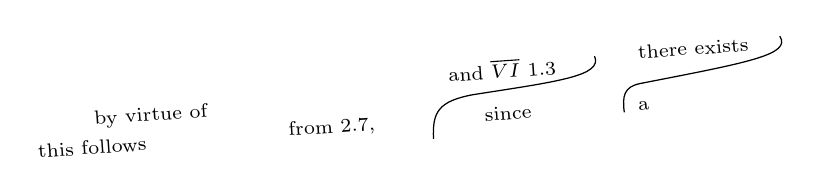
\begin{tikzpicture}[baseline=(correctionbase.base),x=.014cm,y=-.014cm,font=\scriptsize]
\node[anchor=base west,rotate=4] at (270,1578) {\deleted{this follows}};
\node[anchor=base west,rotate=4] at (321,1548) {\inserted{by virtue of}};
\node[anchor=base west,rotate=4] at (497,1558) {from 2.7,};
\node[anchor=base west,rotate=4] at (642,1509) {\deleted{and \(\overline{\text{\uline{VI}}}\) 1.3}};
\node[anchor=base west,rotate=4] at (675,1545) {\deleted{since}};
\node[anchor=base west,rotate=4] at (814,1488) {\inserted{there exists}};
\node[anchor=base west,rotate=4] (correctionbase) at (814,1535) {a};
\draw[line width=.45pt] (783,1485) .. controls (791,1503) and (750,1508) .. (673,1520)
 .. controls (641,1526) and (636,1536) .. (637,1560);
\draw[line width=.45pt] (951,1467) .. controls (962,1484) and (921,1491) .. (824,1510)
 .. controls (810,1513) and (808,1521) .. (810,1536);
\end{tikzpicture} $G\in\mathrm{ob}\,X_{\mathrm{et}}$ \deleted{and} which is \inserted{a scheme} quasi-compact and quasi-separated \deleted{\unsure{and} is} and an epimorphism $G\longrightarrow F$. Now $G$ \deleted{\unsure{as one}} is a quasi-compact object of $\tilde{X}_{\text{ét}}$ (\(\overline{\text{\uline{VII}}}\) 5.6.1), hence $F$ is quasi-compact (\(\overline{\text{\uline{VI}}}\) 1.3), which was to be proved.}

\handwritten{Of course, there would \inserted{have been} reason to recast §§ 1,2 of the present lecture, \inserted{in particular} by linking them \inserted{\deleted{\unsure{explicitly}}} to the general notions of \deleted{the lecture} finiteness of \(\overline{\text{\uline{VI}}}\). We leave this \deleted{\unsure{additional}} task of writing to future generations.}
% archive sheet number: 24
